\documentclass[a4paper]{article}
\linespread{1.6}
\usepackage{floatrow}
\floatsetup[table]{capposition=top}  
\newfloatcommand{capbtabbox}{table}[][\FBwidth] 
\usepackage{enumerate}
\usepackage{comment}
\usepackage{geometry}
\usepackage{setspace}
\usepackage{amsmath}
\usepackage{amssymb}
\usepackage{algorithm}
\usepackage{algorithmicx}
\usepackage{algpseudocode}
\usepackage[pdftex]{graphicx}
\usepackage{float}
\usepackage{subfigure}
\usepackage{listings}


\usepackage{algpseudocode}
\geometry{left=1.2cm,right=1.2cm,top=2.5cm,bottom=2.5cm}

\floatname{algorithm}{Algorithm}
\renewcommand{\algorithmicrequire}{\textbf{Input:}}
\renewcommand{\algorithmicensure}{\textbf{Output:}}

\begin{document}
\begin{spacing}{2.0}
\begin{flushleft}\begin{huge}EEE6512 Image Processing and Computer Vision   Homework 4\end{huge}\end{flushleft}
\begin{flushright}\begin{Large} Hudanyun Sheng \end{Large}\end{flushright}

\section*{\huge\textbf{ Part \uppercase\expandafter{\romannumeral1} Textbook Questions}  }
	\normalsize

	\textbf{4-2} Write the set representation of the binary image $A$, and the array representation of the binary image $B$. 
	$$A = \begin{bmatrix} 1 & 1 & 1 & 0 \\ 0 & 1 & 0 & 0 \\  1 & 1 & 1 & 0 \\ 0 & 0 & 0 & 0 \end{bmatrix}$$
$B = \{(1,1), (2,1), (1,2), (2,2), (3,2), (1,3), (3,3)\}$\\
	Solution:\\ $A = \{(0,0), (1,0), (2,0), (1,1), (0,2), (1,2), (2,2)\}$.\\
	$$B = \begin{bmatrix} 0 & 0 & 0 & 0 \\ 0 & 1 & 1 & 0 \\ 0 & 1 & 1 & 1\\ 0 & 1 & 0 & 1\end{bmatrix}$$
	
	\noindent
	\textbf{4-3} Apply the set operators of Figure 4.2 to the images $A$ and $B$ of the previous question, using $b = (1,1)$. That is, compute $A \cup B$, $A \cap B$, $A_b$, $\check{B}$, $\neg A$, $A\backslash B$. Write the results as arrays. \\
	Solution: \\
	
	\begin{center}
	$A \cup B = \begin{bmatrix} 1 & 1 & 1 & 0 \\ 0 & 1 & 1 & 0 \\ 1 & 1 & 1 & 1\\ 0 & 1 & 0 & 1 \end{bmatrix}$, 	
	$A \cap B = \begin{bmatrix} 0 & 0 & 0 & 0 \\ 0 & 1 & 0 & 0 \\ 0 & 1 & 1 & 0\\ 0 & 0 & 0 & 0 \end{bmatrix}$, 	
	$A_b = \begin{bmatrix} 0 & 0 & 0 & 0 \\ 0 & 1 & 1 & 1 \\ 0 & 0 & 1 & 0\\ 0 & 1 & 1 & 1 \end{bmatrix}$.\\
	$\check{B} =  \begin{bmatrix} 1 & 0 & 1 & 0 \\ 1 & 1 & 1 & 0 \\ 0 & 1 & 1 & 0\\ 0 & 0 & 0 & 0 \end{bmatrix}$,
	$\neg A = \begin{bmatrix}  0 & 0 & 0 & 1 \\ 1 & 0 & 1 & 1 \\ 0 & 0 & 0 & 1\\ 1 & 1 & 1 & 1\end{bmatrix}$, 
	$A\backslash B = \begin{bmatrix} 1 & 1 & 1 & 0 \\ 0 & 0 & 0 & 0 \\ 1 & 0 & 0 & 0\\ 0 & 0 & 0 & 0\end{bmatrix}$\\
	\end{center}
	
	
	\noindent
	\textbf{4-4} Compute Minkowski addition for sets $A_1$ and $B$, as well as Minkowski subtraction for sets $A_2$ and $B$, shown below. Ignore the out-of-bounds pixels. (a) Use the center-in approach. (b) Repeat, using the center-out approach.
	\begin{figure}[H]
	\centering
	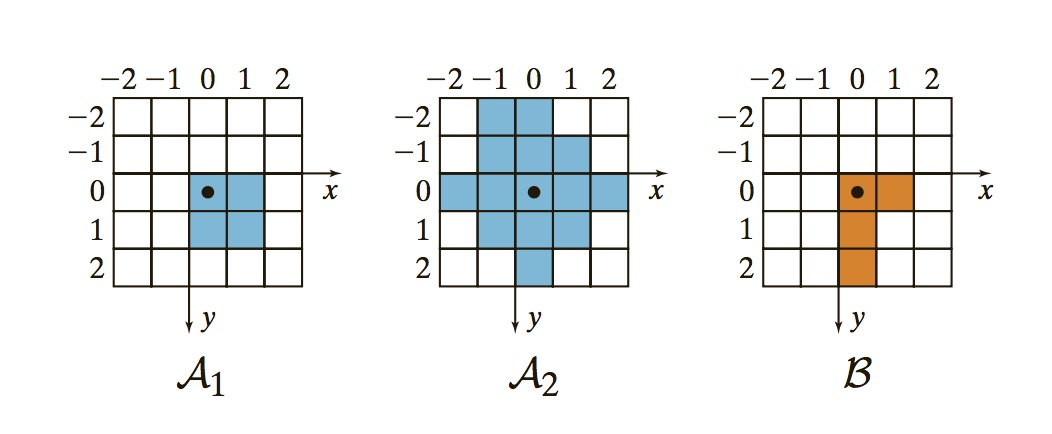
\includegraphics[width = 5in]{1.jpg}
	\end{figure}
	Solution:
	\begin{enumerate}[(a)]
	\item With the center-in approach, the Minkowski addition of sets $A_1$ and $B$ is the union of translation of $A_1$ with its origin places on every $B$, i.e. $A\textcircled{+}b = \bigcup_{b\in B}A_b$. Thus, $A_1\textcircled{+}B =  \{(0,0), (1,0), (2,0), (0,1), (1,1), (2,1), (0,2), (1,2)\}$.\\
		Similarly, the Minkowski addition with the center-in approach: $A\textcircled{-}b = \bigcap_{b\in B}A_b$. Thus, $A_2\textcircled{-}B = \{(-1,0), (0,0), (0,1), (1,1) \}$
	\item With the center-out approach, $A\textcircled{+}B = \{ z: \check{B} \cap A \neq \emptyset\}$, $\check{B} = \{ (0,-2), (0,-1), (0,0), (-1,0)\}$, $A\textcircled{+}b = \bigcup_{b\in B}A_b$. Thus, $A_1\textcircled{+}B =  \{(0,0), (1,0), (2,0), (0,1), (1,1), (2,1), (0,2), (1,2)\}$.\\
	Similarly, with the center-out approach, $A\textcircled{-}B = \{ z: \check{B_z} \in A\}$. \\Thus, $A_2\textcircled{-}B = \{(-1,0), (0,0), (0,1), (1,1) \}$
	\end{enumerate}
		
	\noindent
	\textbf{4-5} What is the difference between erosion and Minkowski subtraction?\\
	The erosion is defined to be Minkowski subtraction after reflecting the structure element.\\
	
	\noindent
	\textbf{4-6} Compute the dilation of the image A below using both center-in and center-out approaches. In both cases, do not reflect the structuring element B. In which approach is reflection necessary to ensure that the output exhibits the same orientation as the input?
	\begin{figure}[H]
	\centering
	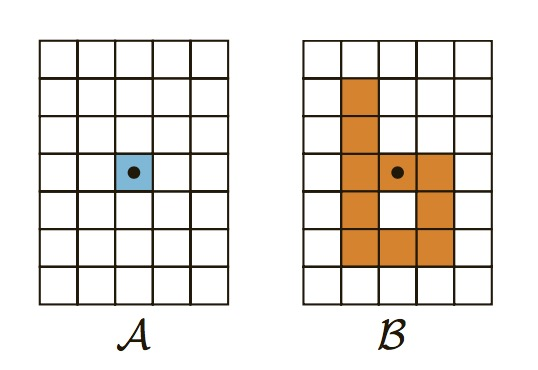
\includegraphics[width = 3in]{2.jpg}
	\end{figure}
	
	Center-in result: 
	\begin{figure}[H]
	\centering
	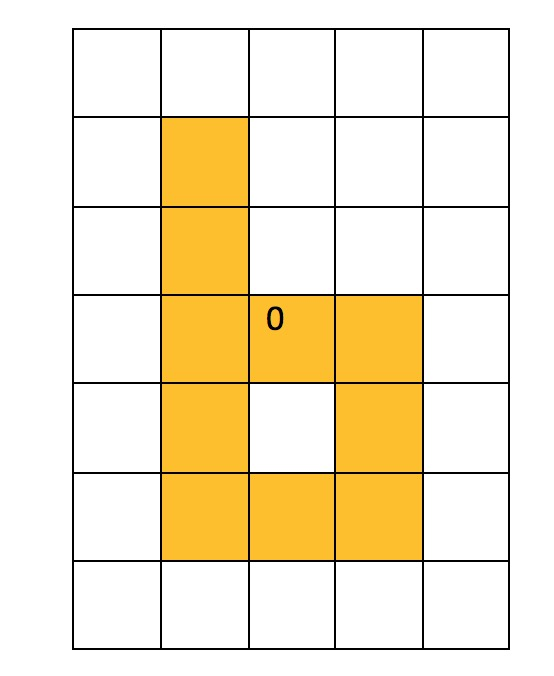
\includegraphics[width = 2in]{centerin.jpg}
	\end{figure}
	
	
	Center-out result: 
	\begin{figure}[H]
	\centering
	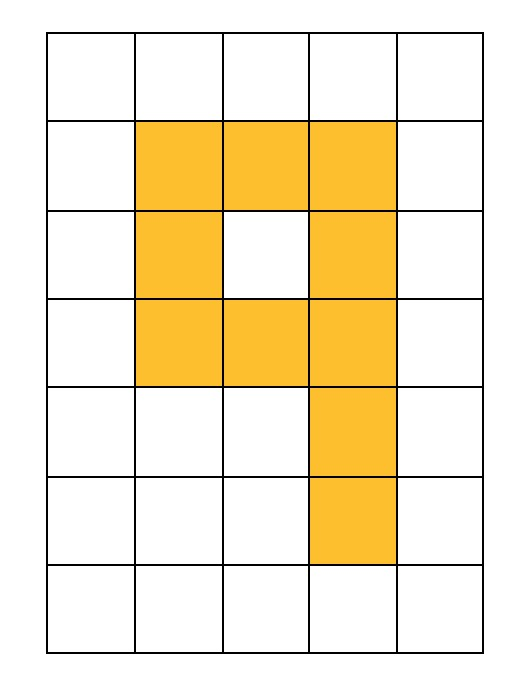
\includegraphics[width = 2in]{centerout.jpg}
	\end{figure}
In center-out approach the reflection is necessary to ensure the output exhibits the same orientation as the input.
		
	\noindent
	\textbf{4-8} Recall the fruit image at the beginning of the chapter, which is reproduced below for convenience. On the two thresholded results shown, identify the name that best describes each of the labeled artifacts A-E: lake, bay, channel, cape, isthmus, or island. Which morphological operator (opening or closing) should be applied to the image on the left to remove noise? To the image on the right?
	\begin{figure}[H]
	\centering
	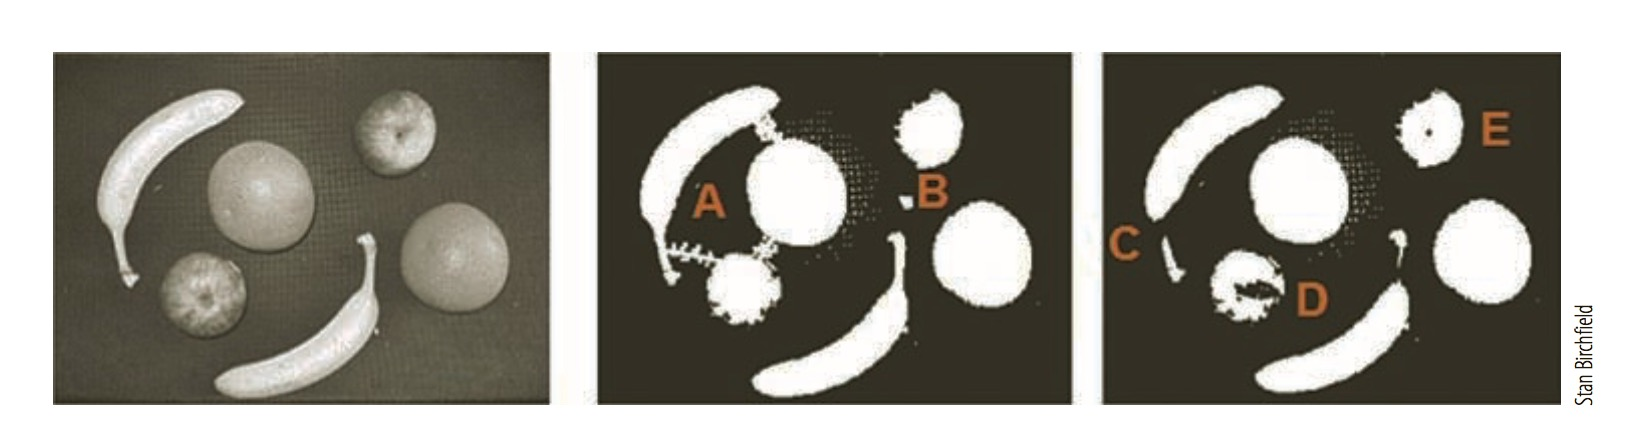
\includegraphics[width = 5in]{3.jpg}
	\end{figure}
	
	A is near several isthmus, B is next to an island, C is next to a channel, D is next to a bay, E is next to a tiny lake.\\
	To remove noise, image open should be applied to the left image, and image close should be applied to the right image.\\


	\noindent
	\textbf{4-12} Which of the labeled pixels below are 4-neighbors of the central pixel c? 8-neighbors? diagonal neighbors? 
	\begin{figure}[H]
	\centering
	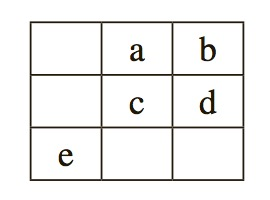
\includegraphics[width = 2in]{4.jpg}
	\end{figure}
	4-neighbors: a, d.\\ 8-neighbors: a, b, d, e. \\ diagonal neighbors: b, e\\
		
	\noindent
	\textbf{4-15} Compute the Euclidean, Manhattan, and chessboard distances from each pixel in a $5\times 5$ image to the central pixel. What shape do the isocontours take in each case?\\
	\begin{comment}
	Euclidean distance: 
	\begin{table}[htbp]
	\begin{tabular}{|c|c|c|c|c|}
	\hline
	$2\sqrt{2}$ & $\sqrt{5}$ & 2 & $\sqrt{5}$ & $2\sqrt{2}$\\
	\hline
	$\sqrt{5}$ & $\sqrt{2}$ & 1 & $\sqrt{2}$ & $\sqrt{5}$\\
	\hline
	2 & 1 & 0 & 1 & 2\\
	\hline
	$\sqrt{5}$ & $\sqrt{2}$ & 1 & $\sqrt{2}$ & $\sqrt{5}$\\
	\hline
	$2\sqrt{2}$ & $\sqrt{5}$ & 2 & $\sqrt{5}$ & $2\sqrt{2}$\\
	\hline
	\end{tabular}
	\end{table}
	
	Manhattan distance: 
	\begin{table}[htbp]
	\begin{tabular}{|c|c|c|c|c|}
	\hline
	4 & 3 & 2 & 3 & 4\\
	\hline
	3 & 2 & 1 & 2 & 3\\
	\hline
	2 & 1 & 0 & 1 & 2\\
	\hline
	3 & 2 & 1 & 2 & 3\\
	\hline
	4 & 3 & 2 & 3 & 4\\
	\hline
	\end{tabular}
	\end{table}
	
	chessboard distance: 
	\begin{table}[htbp]
	\begin{tabular}{|c|c|c|c|c|}
	\hline
	2 & 2 & 2 & 2 & 2\\
	\hline
	2 & 1 & 1 & 1 & 2\\
	\hline
	2 & 1 & 0 & 1 & 2\\
	\hline
	2 & 1 & 1 & 1 & 2\\
	\hline
	2 & 2 & 2 & 2 & 2\\
	\hline
	\end{tabular}
	\end{table}
\end{comment}

\begin{table*} [htbp]
\begin{floatrow}  
\capbtabbox{  
 \begin{tabular}{|c|c|c|c|c|}
 \hline  
$2\sqrt{2}$ & $\sqrt{5}$ & 2 & $\sqrt{5}$ & $2\sqrt{2}$\\
	\hline
	$\sqrt{5}$ & $\sqrt{2}$ & 1 & $\sqrt{2}$ & $\sqrt{5}$\\
	\hline
	2 & 1 & 0 & 1 & 2\\
	\hline
	$\sqrt{5}$ & $\sqrt{2}$ & 1 & $\sqrt{2}$ & $\sqrt{5}$\\
	\hline
	$2\sqrt{2}$ & $\sqrt{5}$ & 2 & $\sqrt{5}$ & $2\sqrt{2}$\\
 \hline  
 \end{tabular}  
}{  
 \caption{Euclidean distance.}  
 \label{tab:tb1}  
}  
\capbtabbox{  
 \begin{tabular}{|c|c|c|c|c|}
 \hline  
	4 & 3 & 2 & 3 & 4\\
	\hline
	3 & 2 & 1 & 2 & 3\\
	\hline
	2 & 1 & 0 & 1 & 2\\
	\hline
	3 & 2 & 1 & 2 & 3\\
	\hline
	4 & 3 & 2 & 3 & 4\\
 \hline  
 \end{tabular}  
}{  
 \caption{Manhattan distance.}  
 \label{tab:tb2}  
}  
\capbtabbox{  
 \begin{tabular}{|c|c|c|c|c|}
 \hline  
	2 & 2 & 2 & 2 & 2\\
	\hline
	2 & 1 & 1 & 1 & 2\\
	\hline
	2 & 1 & 0 & 1 & 2\\
	\hline
	2 & 1 & 1 & 1 & 2\\
	\hline
	2 & 2 & 2 & 2 & 2\\ \hline  
 \end{tabular}  
}{  
 \caption{chessboard.}  
 \label{tab:tb3}  
}  
\end{floatrow}  
\end{table*} 
For Euclidean distance, the isocontours are the circles concentric circles centered in the central pixel; for Manhattan distance, the shape of isocontours are diamonds; for chessboard distance, the shape of isocontours are squares.\\

	\noindent
	\textbf{4-17} Given the following binary image:
	$$I = \begin{bmatrix} 0 & 0 & 1\\ 1 & 0 & 1\\0 & 1 & 1\\\end{bmatrix}$$
	\begin{enumerate}[(a)]
	\item Compute the zeroth-, first-, and second-order regular moments. 
	\item Compute the zeroth-, first-, and second-order central moments. 
	\end{enumerate}
	Solution: $f(2,0) = 1$, $f(0,1) = 1$, $f(2,1) = 1$, $f(1,2) = 1$, $f(2,2) = 1$
	\begin{enumerate}[(a)]
	\item $m_{00} = 2^{0}0^{0}(1) + 0^{0}1^{0}(1) + 2^{0}1^{0}(1) + 1^{0}2^{0}(1) + 2^{0}2^{0}(1) = 5$,\\
	$m_{01} =  2^{0}0^{1}(1) + 0^{0}1^{1}(1) + 2^{0}1^{1}(1) + 1^{0}2^{1}(1) + 2^{0}2^{1}(1) = 6$, $m_{10} = 2^{1}0^{0}(1) + 0^{1}1^{0}(1) + 2^{1}1^{0}(1) + 1^{1}2^{0}(1) + 2^{1}2^{0}(1) = 7$\\
	$m_{02} = 2^{0}0^{2}(1) + 0^{0}1^{2}(1) + 2^{0}1^{2}(1) + 1^{0}2^{2}(1) + 2^{0}2^{2}(1) = 10$, $m_{20} = 2^{2}0^{0}(1) + 0^{2}1^{0}(1) + 2^{2}1^{0}(1) + 1^{2}2^{0}(1) + 2^{2}2^{0}(1) = 13$\\
	$m_{11} =  2^{1}0^{1}(1) + 0^{1}1^{1}(1) + 2^{1}1^{1}(1) + 1^{1}2^{1}(1) + 2^{1}2^{1}(1) = 8$
	\item $\bar x = (2+0+2+1+2)/5 = 1.4$, $\bar y = (0+1+1+2+2)/5 = 1.2$\\
	$\mu_{00} = m_{00} = 5$, $\mu_{10} = \mu_{01}  = 0$, $\mu_{20} = 13 - 1.4\times 7 = 3.2$, $\mu_{02} = 10 - 1.2\times 6 = 2.8$, $\mu_{11} = 8 - 1.2\times 7 = -0.4$.
	\end{enumerate}
		
	

\newpage	
\section*{\huge\textbf{ Part \uppercase\expandafter{\romannumeral2} MATLAB Programming} }
	\normalsize
	The MATLAB code are attached.
		

	
\end{spacing}
\end{document}